\chapter{운동량 모드에서 국소 양자장으로}

양자장이란 무엇이며 입자와는 어떤 관계가 있을까? 기본적인 수학적 도구는 조화 진동자다. 장에는 진동할 수 있는 모드가 여럿 있으며, 장을 양자화한다는 것은 각 모드마다 양자 조화 진동자 하나씩을 두어 함께 구성하는 것이다. 허용되는 모드가 이산적인 목록을 이루는 유한한 주기 공간에서 먼저 살펴보면 이 구성을 가장 쉽게 이해할 수 있다.

\section{주기 공간과 허용되는 파수}

공간 좌표 하나 \(x\)를 택하고 거리 \(L\)만큼 떨어진 점들을 동일시하자. 이 공간은 둘레가 \(L\)인 원으로 생각할 수 있다. 이는 유한 부피를 다룰 때 유용한 기법이다. 양 끝점이 있는 유한 구간에서는 진행파가 끝점에서 반사된다. 주기 구간에서는 반사 없이 어느 방향으로든 계속 진행할 수 있다. 무한 부피에서 생기는 복잡성을 잠시 제거하면서도 병진 대칭, 따라서 운동량 보존을 유지할 수 있다.

평면파는 다음과 같은 형태다.
\begin{equation}
e^{ikx}.
\end{equation}
원을 한 바퀴 돈 뒤에는 원래 값으로 돌아와야 한다. 파동은 \(x=0\)에서 \(1\)와 같으므로 주기성은 다음을 요구한다.
\begin{equation}
e^{ikL}=1.
\end{equation}
왜 \(2\pi\)의 정수배가 이 조건을 만족할까? 오일러 공식에 따르면
\begin{align}
e^{i2\pi n}
&=\cos(2\pi n)+i\sin(2\pi n)\\
&=1,
\qquad n\in\mathbb Z.
\end{align}
몇 주기를 돌더라도 코사인은 \(1\)이고 사인은 \(0\)이기 때문이다. 따라서
\begin{equation}
kL=2\pi n,
\qquad
k=\frac{2\pi n}{L},
\qquad n\in\mathbb Z.
\end{equation}
양은 \(k\)이며 파수라고 한다. 정수 \(n\)는 허용되는 파수를 표시하며, 아직 입자 수를 세는 것은 아니다.

같은 조건을 파장으로 나타낼 수도 있다. 파장이란 위상이 한 주기만큼 진행하는 거리이므로
\begin{equation}
k\lambda=2\pi,
\qquad
k=\frac{2\pi}{\lambda}.
\end{equation}
파장이 길면 파수는 작고, 파장이 짧으면 파수는 크다. 주기성 조건은 원 둘레에 파장이 정수 개 들어맞는다는 뜻이다.

양자역학적 파동의 운동량은
\begin{equation}
p=\frac{h}{\lambda}
=\frac{2\pi\hbar}{\lambda}
=\hbar k.
\end{equation}
따라서 \(k\)와 \(p\)는 \(\hbar\)만큼만 차이가 난다. \(k\)가 양수인지 음수인지에 따라 파동은 서로 반대 방향으로 진행하고 입자의 운동량 방향도 서로 반대가 된다. \(\hbar=1\)로 두는 단위계에서는 별도로 구분하지 않고 \(k\)를 운동량이라고 부르는 것이 일반적이다.

허용되는 각 \(k\) 모드에는 양자가 몇 개든 있을 수 있다. 이에 따라 두 번째 정수가 도입된다.
\begin{equation}
n(k)=\text{number of quanta with wave number }k.
\end{equation}
이를 점유수라고 한다. \(k=2\pi n/L\)의 정수는 모드를 표시하고, \(n(k)\)는 해당 모드에 입자가 몇 개 있는지를 나타낸다. 양수와 음수 \(k\) 모두에 대해 점유수를 지정해야 한다.

\begin{classroomqa}
\lecturetimestamp{00:11:58}
\audiencequestion{\(k\) 자체가 정수인가요?}
\lecturerresponse{아닙니다. 파수는 \(2\pi/L\)의 정수배입니다. 즉 \(k=2\pi n/L\)입니다. 이 식의 정수 \(n\)는 허용되는 운동량을 표시하며, 모드 안의 양자 수를 세는 점유수 \(n(k)\)와는 다릅니다.}
\end{classroomqa}

\section{점유수 상태와 모드 연산자}

양자 상태는 벡터, 즉 선형 공간의 원소다. 상태 벡터끼리 더하거나 수를 곱할 수 있으며, 연산자는 상태 벡터에 작용해 다른 상태 벡터를 만든다. 관측 가능한 실수 물리량은 에르미트 연산자로 나타낸다. 여러 입자의 상태와 장을 모두 선형 결합과 연산자로 구성할 것이므로, 이러한 기본 사항이 여기서 중요하다.

다음을 두자.
\begin{equation}
k_j=\frac{2\pi j}{L},
\qquad j\in\mathbb Z.
\end{equation}
다입자 상태를 표시하는 편리한 방법은 점유수 전체를 하나의 문자열로 나타내는 것이다. 식에 나온 항들을 간단히 \(n_j\equiv n(k_j)\)로 쓰면 다음과 같이 적을 수 있다.
\begin{equation}
\big|\{n(k_j)\}\big\rangle
=
\big|\ldots,n_{-2},n_{-1},n_0,n_1,n_2,\ldots\big\rangle.
\end{equation}
항 \(n(k_1)\)은 첫 번째 양의 운동량 모드에 있는 입자 수이고, \(n(k_2)\)는 두 번째 모드에 있는 입자 수이며, 이런 식으로 계속된다. 이 문자열은 양쪽 방향으로 끝없이 이어진다.

\begin{figure}[t]\centering
\includegraphics[width=0.72\textwidth]{lecture_03_figure_02.png}\caption{허용된 운동량 모드의 점유수 \(n(k)\)}\lectureframe{00:15:04}\end{figure}

각 운동량 모드는 조화 진동자다. 따라서 각 모드에는 올림 연산자와 내림 연산자가 있다. 처음에는 \(a^{+}(k)\)와 \(a^{-}(k)\)로 적었던 표기를 이제 \(a^\dagger(k)\)와 \(a(k)\)로 쓰겠다. 이들의 작용은 다음과 같다.
\begin{align}
a^\dagger(k)\big|\ldots,n(k),\ldots\big\rangle
&=
\sqrt{n(k)+1}\notag\\
&\quad{}\times
\big|\ldots,n(k)+1,\ldots\big\rangle,
\\
a(k)\big|\ldots,n(k),\ldots\big\rangle
&=
\sqrt{n(k)}\,
\big|\ldots,n(k)-1,\ldots\big\rangle.
\end{align}
연산자 \(a^\dagger(k)\)는 \(k\)에 해당하는 슬롯으로 가서 그 점유수를 1만큼 올리고 상태에 \(\sqrt{n(k)+1}\)를 곱한다. 연산자 \(a(k)\)는 같은 슬롯의 점유수를 낮추고 \(\sqrt{n(k)}\)을 곱한다. 허용되는 운동량마다 이런 연산자 쌍이 하나씩 있다.

\begin{figure}[t]\centering
\includegraphics[width=0.58\textwidth]{lecture_03_figure_03.png}\caption{운동량 모드 \(k\)에 대응하는 생성 연산자와 소멸 연산자}\lectureframe{00:17:14}\end{figure}

\section{푸리에 계수에서 연산자로}

이 진동자 연산자와 장의 관계는 보통의 고전적 푸리에 급수에서 시작한다. 주기 구간에서 복소 고전장은 다음과 같이 쓸 수 있다.
\begin{align}
\psi(x)&=\sum_k \alpha(k)e^{ikx},\\
\psi^*(x)&=\sum_k \alpha^*(k)e^{-ikx},
\end{align}
여기서 모든 합은 허용되는 값 \(k=2\pi n/L\)에 대해 취한다. 이는 장을 사인과 코사인으로 전개하는 것과 같다.

복소장에는 실수부와 허수부가 있다. 복소켤레를 취하면 허수부의 부호가 바뀌고, \(e^{ikx}\)는 \(e^{-ikx}\)가 된다. 모든 계수 \(\alpha(k)\)를 지정하면 고전장이 정해진다. \(\alpha(k)\)를 알면 \(\alpha^*(k)\)를 따로 지정할 필요는 없지만, 각 계수의 실수부와 허수부는 서로 독립적인 실수 물리량이다. 이들은 해당 푸리에 성분의 진폭으로 측정할 수 있다. 이런 의미에서 복소 계수 하나에 고전적 관측량 두 개가 담긴다.

양자화하면 이 고전적 푸리에 계수들이 연산자로 바뀐다. 종류가 다른 대상을 등호로 동일시하는 것은 적절하지 않으므로, 대체 규칙으로 쓰는 편이 낫다.
\begin{equation}
\alpha(k)\rightsquigarrow a(k),
\qquad
\alpha^*(k)\rightsquigarrow a^\dagger(k).
\end{equation}
푸리에 부호를 일관되게 정하면 양자장은 다음과 같이 정의된다.
\begin{align}
\Psi(x)&=\sum_k a(k)e^{ikx},\\
\Psi^\dagger(x)&=\sum_k a^\dagger(k)e^{-ikx}.
\end{align}\editorialnote{말로 설명하는 부분에서는 푸리에 부호 규약이 바뀌고, 뒤에서는 그 규약에 의문을 제기한다. 여기서 사용한 켤레쌍은 더 명확하게 제시된 장의 전개식과 위치 상태 계산에서 확인되는 규약이다. 즉 \(\Psi\)에는 \(e^{ikx}\)가, \(\Psi^\dagger\)에는 \(e^{-ikx}\)가 대응한다. 모든 부호를 일관되게 뒤집어도 같은 구성을 나타낸다.}

일단 이것은 정의다. 양자장이란 계수가 연산자인 푸리에 합이다. 더 완전한 정당화를 위해서는 적절한 극한에서 이 연산자들이 고전적 계수를 재현함을 보여야 하며, 그러려면 동역학이 필요하다. 이 문제는 뒤로 미룬다. 지금 분명한 점은 장 자체가 연산자이며, 그 푸리에 계수들 사이의 관계가 조화 진동자의 생성·소멸 관계라는 것이다.

\begin{classroomqa}\lecturetimestamp{00:26:48}\audiencequestion{생성 연산자와 소멸 연산자를 도입하면 동역학이 반드시 입자를 생성하고 소멸시키나요?}\lecturerresponse{아닙니다. 이 연산자들은 점유수를 바꾸는 수학적 연산입니다. 자연 법칙이 실제로 입자 수를 바꾸는지는 동역학에 관한 문제입니다. 동역학이 그런 변화를 허용한다면, 이 연산자들이 이를 기술하는 자연스러운 언어가 됩니다.}\end{classroomqa}

\section{산란과 변하는 입자 수}

먼저 입자 수가 변하지 않는 과정을 생각해 보자. 처음에 존재하는 유일한 입자의 운동량이 \(k_7\)라고 하자. 점유수 표기에서 이 상태는 일곱째 자리에 \(1\)가 있고 나머지 자리는 모두 0이다.
\begin{equation}
|k_7\rangle
=
|\ldots,0,\underset{k_7}{1},0,\ldots\rangle.
\end{equation}
산란 과정에서 입자의 운동량은 \(k_7\)에서 \(k_9\)로 바뀐다. 정확히 이 변화를 일으키는 연산자는 다음과 같다.
\begin{equation}
a^\dagger(k_9)a(k_7).
\end{equation}
가장 오른쪽 연산자가 먼저 작용하여 \(k_7\) 자리에 있는 입자를 제거한다. 이어서 왼쪽 연산자가 \(k_9\) 자리에 입자를 만든다.

\begin{classroomqa}\lecturetimestamp{00:31:37}\audiencequestion{이 \(k_7\to k_9\) 과정에서 제곱근 인자는 어떻게 나타나나요?}\lecturerresponse{\(\sqrt{n(k_7)}=\sqrt{1}=1\)이다. 이를 제거한 뒤 계는 모든 점유수가 0인 상태가 된다. \(k_9\) 모드가 비어 있으므로 생성 인자는 \(\sqrt{n(k_9)+1}=\sqrt{1}=1\)이다. 따라서 이 한 입자 예에서는 두 인자 모두 수치 계수를 바꾸지 않는다.}\end{classroomqa}

두 단계를 차례로 수행해 보자. 소멸시키면
\begin{align}
a(k_7)|k_7\rangle
&=
\sqrt{1}\,|\ldots,0,0,0,\ldots\rangle\\
&=|0\rangle.
\end{align}
점유수가 모두 0인 상태가 진공이다. 입자가 하나도 없는 상태이며, 이 단순한 진동자들의 집합에서는 바닥 상태이기도 하다. 이어서 비어 있는 \(k_9\) 모드에서 생성시키면
\begin{equation}
a^\dagger(k_9)|0\rangle
=\sqrt{0+1}\,|k_9\rangle
=|k_9\rangle.
\end{equation}
따라서
\begin{equation}
a^\dagger(k_9)a(k_7)|k_7\rangle=|k_9\rangle.
\end{equation}
슬롯별로 보면 유일한 \(1\)이 일곱 번째 운동량 모드에서 아홉 번째 모드로 옮겨졌을 뿐이다. 점유수가 한 번도 1을 넘지 않았으므로 두 제곱근 인자는 모두 1이었다. 이미 점유된 모드가 관여하면 이 인자들이 중요해진다.

이 일대일 과정은 보통의 단일 입자 양자역학으로도 기술할 수 있다. 입자 하나의 운동량이 바뀌는 과정이다. 입자 수가 변할 수 있는 경우에는 점유수 언어가 필수적이다. 예를 들어
\begin{equation}
a^\dagger(k_9)a^\dagger(k_{16})a(k_7)|k_7\rangle
=|k_9,k_{16}\rangle
\end{equation}
는 모드 \(k_7\)의 입자 하나가 들어와 모드 \(k_9\)와 \(k_{16}\)에 각각 하나씩 있는 입자 두 개로 바뀌는 수학적 변화를 나타낸다. 표적이 들어오는 입자를 흡수하고 나가는 입자 두 개를 방출하면서 필요한 반동을 모두 받아낼 수 있다. 입자 하나로 제한된 힐베르트 공간에서는 이런 과정을 나타낼 수 없지만, 점유수가 변할 수 있는 상태 공간에서는 자연스럽게 기술된다. 연산자 식 자체가 자연 법칙인 것은 아니다. 입자 수를 바꾸는 법칙을 쓸 때 사용하는 언어다.

\section{점에서의 장 연산자}

위치 공간 연산자 \(\Psi^\dagger(x)\)는 무엇을 생성할까? 양자 상태는 선형 공간을 이루므로 운동량 상태에 복소 계수를 곱해 더하면 새로운 상태를 만들 수 있다. 진공에서 시작하자. 모든 모드가 비어 있으므로
\begin{equation}
\Psi(x)|0\rangle=0.
\end{equation}
우변의 0은 영벡터다. 소멸 연산자가 제거할 입자를 찾지 못하기 때문이다.

켤레 장은 다르게 작용한다.
\begin{align}
\Psi^\dagger(x)|0\rangle
&=\sum_k e^{-ikx}a^\dagger(k)|0\rangle\\
&=\sum_k e^{-ikx}|k\rangle,
\end{align}
여기서
\begin{equation}
|k\rangle=a^\dagger(k)|0\rangle
\end{equation}
는 운동량 \(\hbar k\)인 한 입자 상태다.

\begin{figure}[t]\centering
\includegraphics[width=0.70\textwidth]{lecture_03_figure_05.png}\caption{한 입자 운동량 상태로 전개한 형식적 위치 공간 상태 \(\Psi^\dagger(x)|0\rangle\)}\lectureframe{00:43:16}\end{figure}

형식적으로, 정규화를 무시하면 이 합은 단일 입자 양자역학에서의 일반화된 위치 상태다.\footnote{운동량 모드가 무한히 많으면 정확히 국소화된 위치 상태는 정규화할 수 없다. 대신 유한한 운동량 절단을 적용하고 절단된 합을 정규화하면 \(x\)를 중심으로 날카롭게 국소화된 파동 묶음을 얻는다.}\(e^{-ikx}\)인 계수를 곱한 운동량 고유상태들을 결합하면 \(x\)에 국소화된다. 이런 형식적 의미에서
\begin{equation}
\Psi^\dagger(x)\ \text{creates a particle at position }x,
\end{equation}
한편
\begin{equation}
\Psi(x)\ \text{annihilates a particle at position }x.
\end{equation}
모드 연산자 \(a^\dagger(k)\)는 운동량이 정해진 입자를 생성한다. 장 연산자 \(\Psi^\dagger(x)\)는 형식적으로 \(x\)에 국소화된, 허용되는 운동량 상태들의 결맞은 중첩을 생성한다.

정규화하지 않은 형식적 합에서는 모든 계수 \(e^{-ikx}\)의 크기가 1이다. 유한한 절단을 적용하면 정규화된 절단 상태에서 남아 있는 운동량들의 계수 크기는 서로 같고, 계수의 위상들이 \(x\) 근처에 날카롭게 국소화된 파동 묶음을 만든다. 이것이 양자장과 입자 사이의 기본적인 연결이다.

특수 상대론적 복잡성은 일단 무시하면, 이 모형에서 \(\Psi^\dagger(x)\)는 \(x\)에 입자를 생성한다. 상대론적 장에는 보완이 필요하지만, 연산자값 푸리에 전개와 운동량 모드 연산자와 위치 공간 연산자의 구분은 여전히 기본 개념이다.

\begin{classroomqa}\lecturetimestamp{00:44:59}\audiencequestion{\(x\)는 주기 원 위의 한 점인가요? 원이 커지면 어떻게 되나요?}\lecturerresponse{그렇습니다. 유한 모형에서 \(x\)는 원 위의 한 점이다. 이웃한 허용 파수 사이의 간격은 \(2\pi/L\)이다. \(L\)가 커질수록 간격은 작아지므로, 원하는 운동량마다 그 값에 임의로 가까운 허용값이 존재한다. 무한 부피 극한에서는 \(k\)에 대한 합을 \(k\)에 대한 적분으로 바꾼다. 먼저 이산적인 합을 이해해 두면 유용하다.}\end{classroomqa}

\section{국소적인 입자 반응}

\(\Psi(x)\)와 \(\Psi^\dagger(x)\)가 한 점에서 입자를 소멸시키고 생성하는 것으로 해석되면, 국소성을 직접 표현할 수 있다. \(x\)에 날카롭게 국소화된 표적이 입자를 흡수하는 한편, 나가는 입자 하나는 알파 센타우리 부근에 갑자기 나타나고 다른 하나는 베텔게우스 부근에 나타난다고 상상해 보자. 떨어져 있는 두 사건을 보통의 전파 과정으로 연결할 수 없으므로 이런 반응은 비국소적이다.

요구 조건을 먼저 완화해 나가는 입자들이 표적 주위의 작은 영역 안 어딘가에서 방출되도록 할 수도 있다. 정확한 국소적 이상화는 더 엄격하다. 들어오는 입자가 \(x\)에서 흡수되면 나가는 입자들도 바로 그 점에서 생성된다. 서로 떨어진 점에서 계산한 장들을 사용하는 것은 비국소적인 연산자 곱을 나타낸다. 따라서 국소적인 일대이 연산은 다음과 같다.
\begin{equation}
\Psi^\dagger(x)\Psi^\dagger(x)\Psi(x).
\end{equation}
가장 오른쪽의 장이 \(x\)에서 들어오는 입자를 제거하고, 그 왼쪽의 두 장이 그곳에서 나가는 입자 두 개를 생성한다.\footnote{국소적 일대이 도식은 00:47:38--00:49:13에서 설명한 반응을 따른다.}

\begin{figure}[t]\centering
\begin{tikzpicture}[scale=1.0]
\draw[->] (-2.2,0) -- (0,0);
\fill (0,0) circle (2.2pt);
\draw[->] (0,0) -- (2.0,1.1);
\draw[->] (0,0) -- (2.0,-1.1);
\node at (-1.25,0.3) {$k_{\mathrm{initial}}$};
\node[right] at (0.05,0.05) {$x$};
\node at (1.48,1.34) {$\ell$};
\node at (1.48,-1.34) {$m$};
\end{tikzpicture}\caption{\(x\)에서 들어오는 입자 하나가 흡수되고, 같은 점에서 나가는 입자 두 개가 생성된다.}\end{figure}

들어오는 상태가 파수 \(k_{\mathrm{initial}}\)가 정해진 입자 하나를 포함한다고 하자. 나가는 입자들의 운동량을 구하려면 국소 장의 운동량 공간 전개식을 대입한다. 고정된 운동량 표지와 합의 허수 지표를 구별해야 한다. 다음과 같이 쓰자.
\begin{align}
\Psi(x)&=\sum_q a(q)e^{iqx},\\
\Psi^\dagger(x)&=\sum_\ell a^\dagger(\ell)e^{-i\ell x}.
\end{align}
지표 \(q\)에 대해서는 합을 취하지만, \(k_{\mathrm{initial}}\)는 실제로 점유된 들어오는 모드를 표시한다. \(\Psi^\dagger(x)\)가 두 개 있으므로 서로 독립된 허수 지표, 예컨대 \(\ell\)와 \(m\)를 써야 한다. 같은 지표를 다시 쓰면 서로 독립적인 두 합이 잘못 연결된다. 여기서 \(\ell\)와 \(m\)는 파수이고, \(m\)는 질량을 뜻하지 않는다.

구체적인 그림으로는 \(x\)에 국소화된 원자에 광자 하나가 부딪힌 뒤 광자 두 개가 그 점을 떠나는 과정을 생각할 수 있다. 여기서 사용하는 단순한 장은 완전한 상대론적 광자장보다 비상대론적 입자에 더 적합하므로, 광자라는 표현은 연산자의 계산 방식을 설명하기 위한 것일 뿐이다.

소멸 장이 먼저 작용한다.
\begin{align}
\Psi(x)|k_{\mathrm{initial}}\rangle
&=\sum_q e^{iqx}a(q)a^\dagger(k_{\mathrm{initial}})|0\rangle.
\end{align}
\(q=k_{\mathrm{initial}}\)인 항을 제외한 모든 항은 사라진다. 소멸 연산자는 자기 모드에 있는 입자를 찾아야 하기 때문이다. 따라서
\begin{equation}
\Psi(x)|k_{\mathrm{initial}}\rangle
=e^{ik_{\mathrm{initial}}x}|0\rangle.
\end{equation}
이어서 두 생성 장이 다음과 같이 작용한다.
\begin{align}
&\Psi^\dagger(x)\Psi^\dagger(x)\Psi(x)
|k_{\mathrm{initial}}\rangle
\\
&\quad=
e^{ik_{\mathrm{initial}}x}
\sum_{\ell,m}
e^{-i\ell x}e^{-imx}
a^\dagger(\ell)a^\dagger(m)|0\rangle
\\
&\quad=
\sum_{\ell,m}
e^{i(k_{\mathrm{initial}}-\ell-m)x}
a^\dagger(\ell)a^\dagger(m)|0\rangle.
\end{align}
\(\ell\)와 \(m\)가 서로 다르면 연산자 상태를 \(|\ell,m\rangle\)라고 쓸 수 있다. 두 모드에 입자가 하나씩 들어 있다. 최종 결과는 이런 두 입자 운동량 배치 전체에 대한 합이며, 위상은 들어오는 운동량과 나가는 운동량에 의해 정해진다.

\begin{classroomqa}
\lecturetimestamp{01:00:36}
\audiencequestion{두 생성 연산자는 서로 교환합니까?}
\lecturerresponse{그렇다. 모든 생성 연산자는 서로 교환하고, 모든 소멸 연산자도 서로 교환한다. 생성 연산자와 소멸 연산자는 서로 다른 모드에 대해서는 서로 교환하지만, 같은 모드에 대해서는 교환자가 영이 아니다.}
\end{classroomqa}

\begin{classroomqa}\lecturetimestamp{01:01:34}\audiencequestion{나가는 두 입자의 운동량은 운동량 보존을 만족해야 하나요?}\lecturerresponse{표시된 입자들만 놓고 보면 운동량이 보존되지 않아도 된다. 원자나 표적이 반동할 수 있기 때문이다. 차이 \(k_{\mathrm{initial}}-\ell-m\)는 표적에 전달된 운동량이다. 표적까지 포함한 전체 운동량이 보존되는 양이다.}\end{classroomqa}

계수 \(e^{i(k_{\mathrm{initial}}-\ell-m)x}\)는 순수한 위상이므로 크기가 1이다. 얼핏 보면 모든 쌍 \((\ell,m)\)에 같은 확률 가중치가 붙는 듯하다. 하지만 두 표지가 같을 때는 중요한 단서가 있다.

\(\ell=m\)이면 첫 번째 생성 연산자가 모드 \(m\)에 입자 하나를 넣고, 두 번째 연산자는 이미 입자 하나가 있는 모드에 작용한다.
\begin{align}
a^\dagger(m)a^\dagger(m)|0\rangle
&=a^\dagger(m)|1_m\rangle\\
&=\sqrt{2}\,|2_m\rangle.
\end{align}
따라서 한 모드에 두 입자를 생성하면 진폭에 추가 인자 \(\sqrt{2}\)가 붙는다. 진폭을 제곱하면 확률에는 \(2\)의 인자가 생긴다.

\begin{classroomqa}\lecturetimestamp{01:04:54}\audiencequestion{\(\ell\)와 \(m\)는 생성 계수에 \(n+1\)가 들어가므로 반드시 1만큼 차이가 나야 하나요?}\lecturerresponse{아닙니다. 기호 \(\ell\)와 \(m\)는 운동량 모드를 표시합니다. \(\sqrt{n+1}\)의 \(n\)는 생성 연산자가 작용하는 특정 모드의 점유수입니다. 운동량 표지와 입자 수는 서로 다른 정수입니다.}\end{classroomqa}

\begin{figure}[t]\centering
\includegraphics[width=0.92\textwidth]{lecture_03_figure_06.png}\caption{국소적 일대이 입자 진폭의 운동량 공간 전개}\lectureframe{01:05:44}\end{figure}

이 구성에 나오는 입자들은 서로 동일하다. 따라서 \(\sqrt{2}\)는 첫 번째 입자와 두 번째 입자를 구분하는 표지가 아니라 보손 점유 인자다. 이를 제곱하면 같은 운동량인 경우가 운동량이 서로 다른 단일 항보다 잠정적으로 두 배 더 높은 확률을 갖는 듯하다. 이중 합의 항을 주의 깊게 세어 보면 이 비교를 다시 검토해야 한다.

\begin{classroomqa}\lecturetimestamp{01:06:43}\audiencequestion{복잡한 반응에서는 생성 연산자와 소멸 연산자의 순서를 어떻게 정하나요?}\lecturerresponse{모든 생성 연산자가 왼쪽에, 소멸 연산자가 오른쪽에 놓인 식을 정규 순서라고 한다. 이 형태에서는 가장 오른쪽 연산자들이 먼저 들어오는 입자를 제거하고, 남은 연산자들이 나가는 입자를 생성한다.}\end{classroomqa}

생성 연산자와 소멸 연산자의 혼합 쌍을 서로 바꾸는 것은 일반적으로 단순한 순열이 아니다. 교환자를 사용해야 하며, 같은 모드에서는 추가 항이 생긴다.--\footnote{이 교환자에 관한 단서는 01:0643에서 비형식적으로 설명한 정규 순서화에 대한 편집상 정정이다.}

\begin{classroomqa}\lecturetimestamp{01:07:30}\audiencequestion{운동량 진폭의 크기가 모두 같다면 ``두 배 더 높은 확률''이라는 말은 무슨 뜻인가요?}\lecturerresponse{유한한 공동을 염두에 두자. 공동의 허용 운동량은 이산적이므로 모드별로 확률을 비교할 수 있다. 이 비교는 연속체에서 고립된 점들의 확률을 비교하는 것이 아니다.}\end{classroomqa}

\(\ell\ne m\)인 경우, 제한 없는 이중 합에는 다음 두 순서의 항이 모두 들어간다.
\begin{equation}
a^\dagger(\ell)a^\dagger(m)|0\rangle
\quad\text{and}\quad
a^\dagger(m)a^\dagger(\ell)|0\rangle.
\end{equation}

\begin{classroomqa}\lecturetimestamp{01:08:24}\audiencequestion{\(\ell\ne m\)일 때, 같은 최종 상태가 이중 합에 \((\ell,m)\)와 \((m,\ell)\)로 한 번씩, 총 두 번 나타나나요?}\lecturerresponse{그렇습니다. \(\ell\ne m\)이면 \((\ell,m)\)와 \((m,\ell)\) 항이 모두 들어 있으며, 생성 연산자들이 서로 교환하므로 두 항은 같은 물리적 상태를 나타냅니다.}\end{classroomqa}

두 순서의 항은 서로 같으므로, 정량적으로 채널을 비교하려면 상태 정규화와 이 이중 계수를 먼저 처리해야 한다. 이후 논의에 충분하고 대수적으로 신뢰할 수 있는 결론은 더 제한적이다. 이미 \(n\)개의 동일한 보손이 점유한 모드에서 입자를 생성하면 인자 \(\sqrt{n+1}\)가 생긴다.

\section{자발 방출과 유도 방출}

제곱근 인자를 분명히 보여 주는 더 간단한 예를 살펴보자. \(x\)에 국소화된 물체가 광자 하나를 방출한다고 하자. 광자장이 진공에서 시작하면 나가는 상태는 다음과 같다.
\begin{align}
\Psi^\dagger(x)|0\rangle
&=\sum_k e^{-ikx}a^\dagger(k)|0\rangle\\
&=\sum_k e^{-ikx}|k\rangle.
\end{align}
이 단순화된 모형에서는 모든 운동량의 진폭 크기가 같다. 광자가 하나도 없는 상태에서 일어나는 방출은 자발 방출이다.

이제 \(\ell\) 모드에 광자가 이미 하나 있다고 하자. 같은 국소 생성 장이 작용하면 다음 두 종류의 항이 생긴다.
\begin{equation}
\Psi^\dagger(x)|\ell\rangle
=
\sum_{k\ne\ell}e^{-ikx}|k,\ell\rangle
+e^{-i\ell x}\sqrt{2}\,|2_\ell\rangle.
\end{equation}
\(k\ne\ell\)이면 연산자는 비어 있는 모드에 생성하므로 계수는 \(\sqrt{0+1}=1\)이다. \(k=\ell\)이면 점유된 모드에 생성하므로 계수는 \(\sqrt{1+1}=\sqrt{2}\)이다. 원래 있던 광자는 과정에 영향을 주지 않고 그대로 남는다. 새 광자는 이미 점유된 모드로 방출될 가능성이 더 높다.

\begin{classroomqa}\lecturetimestamp{01:16:14}\audiencequestion{방출을 유도하려면 기존 광자가 같은 위치에 있어야 하나요?}\lecturerresponse{이 단순화된 계산은 두 입자가 한 점에 날카롭게 놓여 있는지가 아니라, 같은 운동량 모드의 점유를 다룬다. 한 입자가 정확한 위치와 정확한 운동량을 동시에 가질 수는 없다. 실제 광자는 파동 묶음으로 기술하지만, 공동 이상화에서는 이산 모드의 운동량이 정해져 있다. 그런 상황에서 방출 증가는 이미 점유된 공동 모드로 일어난다.}\end{classroomqa}

모드 \(\ell\)에 처음에 광자 \(n_\ell\)개가 있으면
\begin{equation}
a^\dagger(\ell)
|\ldots,n_\ell,\ldots\rangle
=
\sqrt{n_\ell+1}
\,|\ldots,n_\ell+1,\ldots\rangle.
\end{equation}
따라서 확률은 \(n_\ell+1\)만큼 증가한다. 광자가 이미 하나 있으면 인자는 \(2\)이다. 모드에 광자가 100개 있으면 진폭 인자는 \(\sqrt{101}\)이고, 그 모드로 방출될 확률은 빈 모드일 때의 \(101\)배다. 보손 모드에 이미 양자가 많을수록 다음 양자가 그 모드로 방출될 가능성이 커진다. 이것이 유도 방출이다.

같은 점유 효과는 산란 반응에도 나타난다. 충돌로 여러 모드에 입자가 생길 수 있다면, 기존 점유는 점유된 모드에서의 생성을 더 유리하게 한다. 이는 원자 붕괴에만 특별히 나타나는 현상이 아니라 이 진동자 대수의 일반적인 성질이다.

\begin{classroomqa}\lecturetimestamp{01:18:15}\audiencequestion{앞서 살펴본 두 입자 과정에서 운동량이 서로 다른 두 입자가 새로 생성되면 여전히 더 큰 가중치가 붙나요?}\lecturerresponse{그렇습니다. 순서가 있는 이중 합에서는 서로 다른 운동량의 쌍이 두 가지 순서로 나타난다. 같은 모드에서 생기는 인자 \(\sqrt{2}\)는 그 조합론적 차이를 줄이지만, 그것만으로 없애지는 않는다.}\end{classroomqa}

앞서와 마찬가지로, 물리적 채널을 비교하려면 일관된 상태 정규화와 계수가 필요하다.

\begin{classroomqa}\lecturetimestamp{01:18:30}\audiencequestion{보손은 이미 점유된 운동량 상태로 끌리는 건가요?}\lecturerresponse{아닙니다. 실제 힘이나 인력은 없다. 이러한 증가는 입자의 동일성과 보손 생성 연산자에 들어 있는 제곱근 인자에서 비롯되는 통계적 결과다.}\end{classroomqa}

두 명칭은 구분해서 기억하면 유용하다. 광자가 없으면 계수는 \(n=0\)에서 시작하며, 이에 따라 자발 방출에 해당하는 단위 인자가 붙는다. 광자가 이미 있으면 인자 \(n+1\) 때문에 그 광자 모드로 방출될 가능성이 더 높아진다. 이것이 유도 방출이다.

고전적인 유사 현상도 있다. 기존 전자기파가 원자를 지나가면 전자를 구동한다. 구동된 전자는 파동이 없을 때보다 더 강하게 복사하며, 추가된 복사는 구동파의 진행 방향과 파수를 따른다. 양자적 설명에서는 기존 파동을 점유된 광자 모드로 대체한다. 이미 있는 양자가 같은 모드에서 양자를 더 생성하도록 유도한다.

이 조화 진동자 대수를 따르는 입자를 보손이라고 한다. 보손은 서로 끌어당겨 그 상태에 모이는 것은 아니지만, 점유된 상태에 쌓이는 통계적 경향을 보인다. 입자에는 보손과 페르미온이라는 두 통계적 종류가 있다. 지금까지의 구성은 보손에 관한 것이며, 반대되는 페르미온의 거동은 뒤에서 다룬다.

\section{보손 대수와 입자 밀도}

각 운동량 모드마다 생성 연산자와 소멸 연산자가 있다. 이들의 대수는 다음과 같다.
\begin{align}
[a^\dagger(k),a^\dagger(\ell)]&=0,\\
[a(k),a(\ell)]&=0,\\
[a(k),a^\dagger(\ell)]&=\delta_{k\ell}.
\end{align}
여기서
\begin{equation}
[A,B]=AB-BA,
\end{equation}
이며 크로네커 델타는 다음과 같다.
\begin{equation}
\delta_{k\ell}=
\begin{cases}
1,&k=\ell,\\
0,&k\ne\ell.
\end{cases}
\end{equation}
운동량이 같든 다르든 생성 연산자끼리는 서로 교환하며, 소멸 연산자끼리도 마찬가지다. 생성 연산자와 소멸 연산자는 운동량이 다르면 서로 교환하고, 운동량이 같으면 익숙한 단일 진동자의 교환자 관계를 따른다.

\(\Psi(x)\)의 푸리에 정의와 함께 이 관계들은 가장 단순한 보손 양자장을 정의한다. 장의 역할은 모드별로, 또는 지정된 위치에서 입자를 생성하고 소멸시키는 것이다.

이제 다음 연산자를 생각해 보자.
\begin{equation}
\int_0^L dx\,\Psi^\dagger(x)\Psi(x).
\end{equation}
미리 이름을 붙이는 대신 직접 계산해 보자. 푸리에 전개식을 대입하면 다음과 같다.
\begin{align}
\int_0^L dx\,\Psi^\dagger(x)\Psi(x)
&=
\sum_{k,\ell}a^\dagger(k)a(\ell)
\int_0^L dx\,e^{-ikx}e^{i\ell x}
\\
&=
\sum_{k,\ell}a^\dagger(k)a(\ell)
\int_0^L dx\,e^{i(\ell-k)x}.
\end{align}
\(k=\ell\)이면 지수함수는 \(1\)이고 적분값은 \(L\)이다. \(k\ne\ell\)이면 원을 따라 사인과 코사인의 주기가 정수 번만큼 적분되므로 양의 부분과 음의 부분이 상쇄된다. 따라서
\begin{equation}
\int_0^L dx\,e^{i(\ell-k)x}=L\delta_{k\ell}.
\end{equation}
이중 합은 다음과 같이 간단해진다.
\begin{equation}
\int_0^L dx\,\Psi^\dagger(x)\Psi(x)
=L\sum_k a^\dagger(k)a(k).
\end{equation}
각 모드에서
\begin{equation}
a^\dagger(k)a(k)=N_k
\end{equation}
은 점유수 연산자다. 이를 모두 더하면 전체 입자 수를 센다.
\begin{equation}
N=\sum_k N_k=\sum_k a^\dagger(k)a(k).
\end{equation}
현재 사용하는 푸리에 정규화에서는
\begin{equation}
N=\frac{1}{L}\int_0^L dx\,
\Psi^\dagger(x)\Psi(x).
\end{equation}
다른 관례에서는 \(1/\sqrt{L}\) 같은 인자를 푸리에 전개식에 넣고 여기서 명시적으로 나타나는 \(1/L\)을 없앤다. 여기서 사용하는 관례에 따른 국소 입자 수 밀도 연산자는 다음과 같다.
\begin{equation}
\rho(x)=\frac{1}{L}\Psi^\dagger(x)\Psi(x),
\qquad
\int_0^L dx\,\rho(x)=N.
\end{equation}
따라서 \(\Psi^\dagger(x)\Psi(x)\)은 입자 밀도에 비례한다. 이를 수학적으로 한 점에 있는 입자의 수라고 부르는 것은 오해를 부르며, 국소적인 양은 밀도로 나타내는 것이 적절하다.

전체 입자 수는 보존될 수도 있고 보존되지 않을 수도 있다. 동역학이 입자를 생성하거나 흡수하면 \(N\)은 시간에 따라 변할 수 있다. 동역학에서 입자 수가 보존된다면 \(N\)은 보존되는 관측량이다.

모드 연산자들의 교환자를 알면 \(\Psi(x)\)와 \(\Psi^\dagger(x)\)의 교환자도 계산할 수 있다. 이 계산은 푸리에 합을 적용하는 유익한 연습문제로 남겨 둔다.

이 구성은 동일한 보손 한 종류를 설명한다. 동일하다는 것은 입자들이 모두 같은 종류라는 뜻이며, 위치와 운동량은 서로 달라도 된다. 전자와 광자를 같은 장 \(\Psi\)에 넣을 수는 없다. 광자장에는 이 기초 모형을 상대론적으로 확장해야 한다. 전자장에는 다른 페르미온 대수가 필요하다.

\begin{classroomqa}\lecturetimestamp{01:35:43}\audiencequestion{이 구성은 1차원에만 해당하나요?}\lecturerresponse{지금까지의 예에는 공간 좌표가 하나 있지만, 본질적인 내용은 차원 수에 달려 있지 않습니다. 좌표와 운동량 성분을 추가하면 더 높은 차원으로 확장할 수 있습니다.}\end{classroomqa}

\editorialnote{여기서 이어지는 짧은 문답은 형광과 유도 방출로 시작해 투명성과 간섭으로 넘어가는 듯하다. 손상된 문구만으로는 질문이나 답변을 신뢰성 있게 복원할 수 없다.}

예로는 광자, 힉스 보손, 중력자가 있다.\footnote{짧은 예시 목록에 나온 다른 입자 이름은 식별하기 어려워 남기지 않았다.}

\section{큰 점유수와 고전장 극한}

복소 장 연산자 자체는 하나의 에르미트 관측량이 아니다. 그 두 에르미트 성분은 다음과 같다.
\begin{equation}
\Psi_1(x)=\frac{\Psi(x)+\Psi^\dagger(x)}{2},
\quad
\Psi_2(x)=\frac{\Psi(x)-\Psi^\dagger(x)}{2i}.
\end{equation}
이들은 고전장의 실수부와 허수부에 대응하는 양자적 유사물이다. 두 성분은 서로 교환하지 않으므로 임의의 정밀도로 동시에 측정할 수 없다. 이는 조화 진동자의 켤레 변수 사이 불확정성에 대응하는 장의 경우다.

그렇다면 장은 언제 고전적인 파동처럼 거동할 수 있을까? 크게 들뜬 하나의 운동량 모드 \(k\)를 생각해 보자. 그 모드의 수 연산자는
\begin{equation}
a^\dagger(k)a(k)=N_k.
\end{equation}
이다. 상태의 평균 점유수가 크다고 하자. 즉, \(\langle N_k\rangle=n_k\gg 1\)이다. 그러면 거시적 진폭의 척도는 대략 \(\sqrt{n_k}\)이다. 한편
\begin{equation}
[a(k),a^\dagger(k)]=1
\end{equation}
의 우변은 일정하게 유지된다. 교환자는 결코 사라지지 않지만, 점유수가 클 때에는 그 효과가 들뜸의 제곱 척도에 비해 작을 수 있다. 큰 점유수는 고전적 극한에 필요한 척도를 제공하지만, 그것만으로 충분하지는 않다. 두 사분면의 불확정성이 거시적 장 진폭에 비해 작도록 상태의 위상도 적절히 결맞아 있어야 한다.\footnote{이 점은 큰 점유수에 관한 경험칙에 조건을 붙인다. 수 고유상태에서는 \(\langle a(k)\rangle=0\)이므로 위상이 정해져 있지 않고, 사분면 요동은 \(\sqrt{n_k}\) 정도이다. 따라서 수 고유상태만으로는 고전적인 파동이 되지 않는다.}

전자기장에서 큰 점유수란 광자가 많다는 뜻이다. 관련 모드에 광자가 많고 위상 결맞음이 적절한 상태에서는 측정 가능한 장 성분이 보통의 고전 전자기파처럼 근사적으로 거동한다. 광자가 몇 개뿐이면 양자의 불연속성이 드러나 고전파 기술은 성립하지 않는다. 어느 영역에서든 양자장은 연산자로 남으며, 달라지는 것은 양자 요동이 상대적으로 얼마나 중요한가이다.

\begin{classroomqa}\lecturetimestamp{01:42:09}\audiencequestion{큰 점유수란 초기 점유수인가요, 최종 점유수인가요?}\lecturerresponse{이 과정에서 광자 수가 조금만 변한다면 이 논의에서는 어느 쪽인지 중요하지 않습니다. 초기 점유수와 최종 점유수는 모두 크고, 두 점유수의 차이는 어느 쪽에 견주어도 작습니다.}\end{classroomqa}

그 반대 극단은 모든 점유수가 0인 바닥 상태다. 이 상태는 양자적 성격이 매우 강하며, 표기할 때 영벡터와 혼동하지 않도록 주의해야 한다.

\begin{classroomqa}\lecturetimestamp{01:42:36}\audiencequestion{소멸 연산자가 진공에 작용하면 진공을 다시 만드는 건가요, 아니면 아무 상태도 만들지 않나요?}\lecturerresponse{영벡터 \(a(k)|0\rangle=\mathbf{0}\)를 만든다. 진공 \(|0\rangle\)은 입자가 없는 실제 정규화 상태이며 \(\langle0|0\rangle=1\)를 만족한다. 진공은 영벡터가 아니다. 영벡터의 노름은 0이며 물리적 상태를 나타내지 않는다.}\end{classroomqa}

\begin{classroomqa}\lecturetimestamp{01:44:11}\audiencequestion{장 자체도 또 다른 종류의 상태인가요?}\lecturerresponse{아니다. 양자장론에서 장은 연산자다. 상태는 벡터이며 장 연산자는 그 벡터에 작용한다.}\end{classroomqa}

\section{주기 공간의 실제 적용}

주기 조건을 이용한 구성은 계산상의 장치이지, 우주가 어떤 특정한 둘레를 가진 원이라고 주장하는 것이 아니다. 이와 밀접한 이산 모드 계는 실제로 존재한다.

\begin{classroomqa}\lecturetimestamp{01:45:03}\audiencequestion{유한한 주기 모형은 실제로 어떻게 쓰이나요?}\lecturerresponse{반사벽이 있는 공동 속 복사는 익숙한 이산 모드 집합을 제공한다. 닫힌 고리 모양의 전선을 따라 움직이는 입자는 직접적인 주기성의 예다. \(L\)을 우주의 크기로 잡을 필요도 없고, 특별히 유용하지도 않다.}\end{classroomqa}

\(L\)를 고정하면 인접한 운동량 사이의 간격은 0이 아니지만, 운동량의 개수가 유한해지는 것은 아니다.

\begin{classroomqa}\lecturetimestamp{01:45:39}\audiencequestion{길이 \(L\)을 고정하면 가능한 운동량 상태의 총수가 제한되나요?}\lecturerresponse{아니다. 허용되는 값은 \(k_j=2\pi j/L\)이고, \(j\)는 임의의 정수일 수 있으므로 모드는 여전히 무한히 많다. 유한한 \(L\)이 유한 개의 모드만 남기는 것은 선택한 최대 운동량보다 낮은 범위에서뿐이다. 그런 절단을 두지 않으면 운동량 표지는 계속 무한히 커질 수 있다.}\end{classroomqa}

진동자 해석은 반대 방향으로도 생각할 수 있다. 기초적인 진동자 역학에서는 켤레 변수에서 출발해 \(a\)와 \(a^\dagger\)를 구성한다. 여기서는 모드 연산자를 먼저 도입했으므로, 그 켤레 변수는 어디에 나타나는지 묻는 것이 자연스럽다.

\begin{classroomqa}\lecturetimestamp{01:46:43}\audiencequestion{고정된 모드에서, \(a(k)\)와 \(a^\dagger(k)\)로부터 시작하는 구성에서는 진동자 변수 \(X\)와 \(P\)에 해당하는 것이 무엇인가요?}\lecturerresponse{고정된 각 운동량 모드에는 진동자 하나가 있다. 그 두 에르미트 직교 성분은 \(a(k)\)와 \(a^\dagger(k)\)로 구성되며, 실수부와 허수부인 장 성분이 \(\Psi\)와 \(\Psi^\dagger\)로 구성되는 것과 같다. 정규화와 명칭을 서로 바꿀 가능성을 제외하면, 이들은 \(X\)와 \(P\)에 대응한다.}\end{classroomqa}

고정된 모드의 경우, 관례에 따라 달라지는 수치 계수를 생략하면 쿼드러처는\footnote{ 이 대목은 01:46:43 한 운동량 모드와 전체 장 사이를 다소 느슨하게 오간다. 제시된 관계식은 고정 모드에 대한 진술을 명시적으로 보여 준다. \(\Psi(x)\)와 \(\Psi^\dagger(x)\)는 모든 모드에 대한 푸리에 합이다.}
\begin{equation}
X_k\propto a(k)+a^\dagger(k),
\qquad
P_k\propto \frac{a(k)-a^\dagger(k)}{i}.
\end{equation}
앞서 도입한 위치 공간 성분 \(\Psi_1(x)\)와 \(\Psi_2(x)\)는 이러한 모드 쿼드러처의 푸리에 중첩이며, 하나의 고정된 모드에 대한 쿼드러처는 아니다. 이들의 불확정성 관계는 약하게 들뜬 양자장을 완전히 고전적인 대상으로 간주하려 할 때 마주치는 것과 같은 장애물이다.

\section{고차원에서의 주기 공간}

\begin{classroomqa}\lecturetimestamp{01:48:21}\audiencequestion{주기 공간은 1차원보다 높은 차원에서 어떻게 나타내나요?}\lecturerresponse{2차원에서 원에 해당하는 것은 토러스다. 왼쪽 변과 오른쪽 변을 서로 동일시하고 아래쪽 변과 위쪽 변도 서로 동일시하는 직사각형으로 나타낼 수 있다. 주기 방향이 두 개이므로 운동량 성분 둘 다 양자화된다.}\end{classroomqa}

토러스는 흔히 도넛 표면으로 그려지지만, 계산에는 직사각형이 더 편리하다. 표면을 한 번 잘라 원기둥 모양으로 펼친다. 원기둥을 한 번 더 잘라 평평하게 펼친다. 이렇게 얻은 직사각형에는 여전히 두 쌍의 변이 서로 동일시되어 있다. 왼쪽 변은 오른쪽 변과 같고, 아래쪽 변은 위쪽 변과 같다.\footnote{직사각형과 두 쌍의 변을 동일시하는 조건, 입자가 다시 나타나는 방식, 두 운동량 성분이 모두 양자화된다는 설명은 01:48:46--01:50:58를 따른다. \(k_x\)와 \(k_y\)에 대한 제시된 식은 앞서의 조건 \(kL=2\pi n\)을 각 성분에 적용해 다시 쓴 것이다.}

입자가 오른쪽 변을 지나면 왼쪽 변의 대응하는 지점에 다시 나타난다. 위쪽 변을 지나면 아래쪽 변의 대응하는 지점에 다시 나타난다. 주기적인 장은 다음 조건을 만족한다.
\begin{align}
\Psi(x+L_x,y)&=\Psi(x,y),\\
\Psi(x,y+L_y)&=\Psi(x,y).
\end{align}
평면파 \(e^{i(k_x x+k_y y)}\)에 이 동일시 조건을 적용하면 다음을 얻는다.
\begin{equation}
k_x=\frac{2\pi n_x}{L_x},
\qquad
k_y=\frac{2\pi n_y}{L_y},
\qquad
n_x,n_y\in\mathbb Z.
\end{equation}
운동량의 두 성분 모두 이산적이다.

\begin{figure}[t]\centering
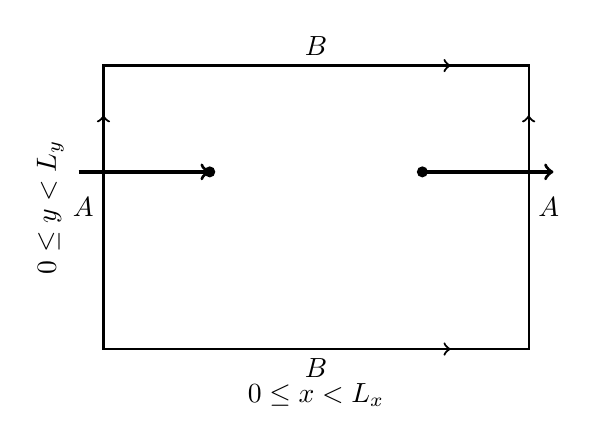
\begin{tikzpicture}[x=0.9cm,y=0.9cm]
\draw[thick] (0,0) rectangle (6,4);
\draw[->,thick] (0,0.7) -- (0,3.3);
\draw[->,thick] (6,0.7) -- (6,3.3);
\draw[->,thick] (1.1,0) -- (4.9,0);
\draw[->,thick] (1.1,4) -- (4.9,4);
\node[left] at (0,2) {$A$};
\node[right] at (6,2) {$A$};
\node[below] at (3,0) {$B$};
\node[above] at (3,4) {$B$};
\draw[->,very thick] (4.5,2.5) -- (6.35,2.5);
\draw[->,very thick] (-0.35,2.5) -- (1.5,2.5);
\fill (4.5,2.5) circle (2pt);
\fill (1.5,2.5) circle (2pt);
\node at (3,-0.65) {$0\leq x<L_x$};
\node[rotate=90] at (-0.75,2) {$0\leq y<L_y$};
\end{tikzpicture}\caption{2차원 주기 공간. 같은 표지가 붙은 변끼리 동일시되므로, 입자가 한 변을 통과하면 맞은편 변의 대응하는 지점에 다시 나타난다.}\end{figure}

\begin{classroomqa}\lecturetimestamp{01:50:58}\audiencequestion{주기 조건을 부여하는 대상은 공간인가요, 공간 속 물체인가요?}\lecturerresponse{공간에 부여한다. 물체와 장은 그 공간에 존재하며 공간의 동일시 조건을 따른다. 무한 부피 문제를 다루기 쉽게 하려고 주기 조건을 부여한 뒤, 부피를 크게 하고 운동량 합을 적분으로 바꾸어 그 조건을 제거한다.}\end{classroomqa}

3차원에 해당하는 것은 마주 보는 세 쌍의 면을 서로 동일시한 정육면체이다. 왼쪽 면과 오른쪽 면이 같고, 위쪽 면과 아래쪽 면이 같으며, 앞쪽 면과 뒤쪽 면도 같다. 입자가 어느 면을 지나가든, 그 면과 동일시된 반대편 면으로 다시 나타난다.\footnote{주기적인 정육면체와 세 쌍의 동일시된 면은 01:51:27--01:52:17를 따른다. \(k_i\)에 대한 제시된 방정식은 세 주기 방향에 적용한 앞서의 조건 \(kL=2\pi n\)을 각 성분별로 다시 쓴 것이다.}세 운동량 성분은 다음을 만족한다.
\begin{equation}
k_i=\frac{2\pi n_i}{L_i},
\qquad i=x,y,z,
\end{equation}
각 방향마다 정수 \(n_i\)가 하나씩 있다. 같은 규칙으로 임의의 차원에서 토러스를 정의할 수 있다.

\begin{figure}[t]\centering
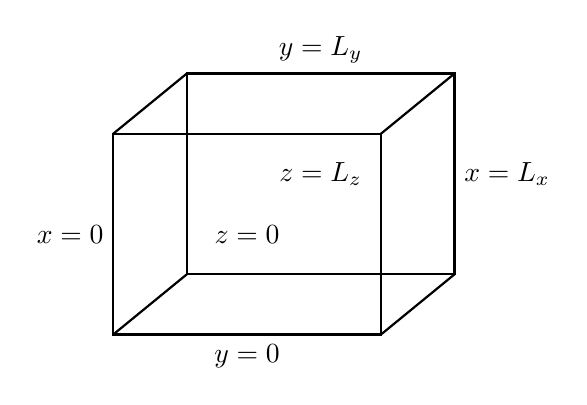
\begin{tikzpicture}[scale=0.85]
\draw[thick] (0,0) rectangle (4,3);
\draw[thick] (1.1,0.9) rectangle (5.1,3.9);
\draw[thick] (0,0) -- (1.1,0.9);
\draw[thick] (4,0) -- (5.1,0.9);
\draw[thick] (4,3) -- (5.1,3.9);
\draw[thick] (0,3) -- (1.1,3.9);
\node[left] at (0,1.5) {$x=0$};
\node[right] at (5.1,2.4) {$x=L_x$};
\node[below] at (2,0) {$y=0$};
\node[above] at (3.1,3.9) {$y=L_y$};
\node at (2,1.5) {$z=0$};
\node at (3.1,2.4) {$z=L_z$};
\end{tikzpicture}\caption{각 쌍의 마주 보는 면을 서로 동일시한 정육면체로 나타낸 3차원 주기 공간.}\end{figure}

\begin{classroomqa}\lecturetimestamp{01:52:20}\audiencequestion{장론에서는 공간의 격자 간격을 물리적으로 정하나요?}\lecturerresponse{그것은 추측에 관한 질문이다. 여기서 실용적인 목적에 한해서는 공간을 연속으로 다룬다. 양자는 입자이지 공간 격자의 칸이 아니다. 원을 이용한 구성에서 이산화되는 것은 운동량이며, 위치는 연속이고 주기적이다.}\end{classroomqa}

\editorialnote{격자 간격을 논의하는 중 손상된 긴 대목에는 플랑크 규모가 언급되지만, 공간의 근본적인 불연속성에 관한 주장을 복원할 수 있을 만큼 문구가 남아 있지 않다. 여기서는 그런 주장을 추론하지 않는다.}

\(k\)의 이산성은 전적으로 주기적 파동함수를 부과한 데서 비롯되었다. 좌표 \(x\) 자체가 격자 위에 놓인다는 증거는 아니다. 공간에 근본적인 미시 구조가 있을 수 있는지 묻는 것은 타당하지만, 이는 별개의 추측성 문제다.

\section{페르미온과 외부장}

보손 모드는 임의의 음이 아닌 점유수를 허용한다. 페르미온에는 반대 성질이 요구된다. 파울리 배타 원리는 동일한 페르미온 두 개가 같은 상태를 차지하는 것을 금지한다.

\begin{classroomqa}\lecturetimestamp{01:55:13}\audiencequestion{교환자를 반교환자로 바꾸면 가장 간단한 페르미온 이론이 되나요?}\lecturerresponse{요점만 말하면 그렇다. 교환자는 \([A,B]=AB-BA\)이고, 반교환자는 \(\{A,B\}=AB+BA\)이다. 이에 대응하는 페르미온 생성 및 소멸 대수는 파울리 배타 원리를 구현하므로, 이미 점유된 상태에 동일한 페르미온을 하나 더 넣을 수 없다. 자세한 이론은 뒤에서 다룬다.}\end{classroomqa}

두 곱은 부호가 다르다.
\begin{equation}
[A,B]=AB-BA,
\qquad
\{A,B\}=AB+BA.
\end{equation}
교환자는 두 연산자를 맞바꾸면 부호가 바뀌는 반면, 반교환자는 대칭이다. 반교환자가 0이면 다음이 성립한다.
\begin{equation}
\{A,B\}=0
\quad\Longrightarrow\quad
AB=-BA.
\end{equation}
이러한 한 쌍에서는 두 페르미온 연산자를 맞바꾸면 부호가 바뀐다. 이는 보통의 교환보다 더 낯선 성질이다. 보통의 교환에서는 \([A,B]=0\)이면 \(AB=BA\)이다. 보손의 교환자를 이에 대응하는 반교환 대수로 바꾸는 것이 페르미온으로 이어지는 수학적 변화이며, 그 자세한 전개는 뒤로 미룬다.

반교환은 보손에서 보이는 통계적 거동과 반대다. 동일한 페르미온이 한 모드에 자극을 받아 계속 쌓이는 일은 없다. 그 모드가 점유되어 있으면 동일한 페르미온이 더 들어올 수 없다. 하나의 페르미온 상태에는 동일한 페르미온을 최대 하나만 둘 수 있으므로, 그 한 상태에 임의로 많은 페르미온을 넣어 고전장 극한을 얻을 수는 없다.

\begin{classroomqa}\lecturetimestamp{01:58:03}\audiencequestion{알파 입자는 페르미온으로 이루어졌는데 어떻게 보손일 수 있나요?}\lecturerresponse{짝수 개의 페르미온 구성 입자가 결합한 복합 입자는 보손 통계를 따를 수 있다. 이런 복합 보손 여러 개를 같은 전체 상태에 두는 것은 각각의 페르미온 구성 입자를 동일한 하나의 단일 입자 상태에 두는 것과 다르다.}\end{classroomqa}

복합 입자의 통계는 결합된 물체 전체의 성질이다. 따라서 페르미온 구성 입자들은 그 구성 입자에 대한 배타 원리를 위반하지 않으면서 보손처럼 거동하는 물체를 이룰 수 있다.

\begin{classroomqa}\lecturetimestamp{01:58:33}\audiencequestion{외부장은 어떻게 포함하나요?}\lecturerresponse{지금까지의 구성에는 외부 배경장이 포함되지 않았다. 그런 장은 고전장으로 주어질 수도 있고, 많은 양자가 들어 있는 상태로 표현할 수도 있다.}\end{classroomqa}

두 설명이 일치하려면 큰 점유수 상태를 적절히 준비하고 위상 결맞음을 갖춰야 한다. 입자 수만으로는 충분하지 않다.\footnote{이 문답은 많은 양자가 있을 때의 규모를 제시한다. 여기서는 큰 점유수만으로 고전장을 보장한다고 오해하지 않도록 위상 결맞음을 추가 조건으로 명시한다.}그런 반고전적 영역에서는 양자 효과에 따른 작은 편차를 제외하면 두 설명의 효과가 일치한다. 이는 기본적인 일관성 조건이다. 개별 양자가 중요할 때 전자기장은 이산적인 광자를 기술해야 하는 동시에, 광자가 많고 위상 결맞음이 적절한 상태에서는 익숙한 고전 전자기파의 작용을 재현해야 한다.
